\chapter{Multi-Agent Systems for Optimization and the AMAS Theory}\label{AMAS_chapter}

As stated in our conclusion on optimization, providing a method able to scale to the needs of the full range of optimization problems will requires it to be capable of adapting to the problem at hand.

The main theme of the SMAC team\footnote{\emph{Systèmes Multi-Agents Coopératifs} (Cooperative Multi-Agent Systems)\\\url{http://irit.fr/-Equipe-SMAC-}}, in which this thesis has been realized, is the Adaptive Multi-Agent Systems (AMAS) Theory. This theory relates to the design of agent-based complex systems with self-adaptive capabilities.

In this chapter we will first describe what multi-agent systems are and how they can be used for problem solving, before concentrating on the concepts of the AMAS theory.

\section{Multi-Agent Systems}

Multi-Agent Systems (MAS) are a relatively recent field which can be seen as the intersection of Artificial Intelligence (AI) and Systems Theory. Several specific subfields of AI have been defined, among which we can find automated problem solving, machine learning, robotics, knowledge engineering, planning, affective computing \emph{etc.}. As a reminder, the AI field was developed in 1950s as \enquote{the science and engineering of making intelligent machines}, as stated by McCarthy, one of the pioneers of the field \cite{mccarthy2006proposal}. This rather ambitious project was somewhat toned down during the 70s when the field was the subject of several setbacks leading to an \enquote{AI winter} \cite{10.1109/MIS.2008.20}, which effects can still be felt today. The commonly accepted reason for this setback was that the researchers had been too optimistic in their expectations of the breakthroughs which would be produced by the field, and did not take enough into account the inherent complexity of some of the tasks they were proposing to handle (\emph{e.g. language processing}).

This disgrace period of the AI field ended with the success of expert systems in the 80s. These systems aim to emulate the ability of a human being to take decisions based on expert knowledge, using inference mechanisms (via an \emph{inference engine}) and a rules database.
However, even expert systems cannot avoid the complexity of modeling knowledge, and are still ultimately limited by the growth of their rules database. This concern, among others (such as privacy of informations) led to a new field of AI named Distributed Artificial Intelligence (DAI) \cite{o1996foundations}, where several expert systems collaborate to provide a collective diagnostic of a situation.

In parallel to the developments of AI, another field of knowledge emerged in the beginning of the century, Cybernetics (also called System Theory), the study of self-regulating systems. Interestingly, this field had radically different origins from AI, taking root in social and natural sciences. These two disciplines had a somewhat uneasy coexistence for some times during the 50s, after which AI took the lead and cybernetics was somewhat relegated in the background (on this topic, see for example \cite{5/2/086.cariani}). The field knew a revival in the 70s with the \enquote{new cybernetics}, or \enquote{second-order cybernetics}, which introduces the study of self-organizing systems and the notion of observer.

It is interesting to note the conflicting nature of AI and cybernetics. AI initially based itself on a reductionist approach of knowledge, using symbol manipulation coming from algebra and logics. Cybernetics was part of the more general epistemological upheaval of Constructivism.

It is at the conjunction of these two seemingly contradictory fields that was born the study of Multi-Agent Systems.

\subsection{Principles of Multi-Agent System}

Before talking about MAS, we must explain the notion of \emph{agent}. Several definitions of what is an agent have been proposed. We keep here the (mostly) consensual one proposed by Wooldridge in \cite{wei1999mutiagent}:

\definition{Agent}{\enquote{An \emph{agent} is a computer system that is \emph{situated} in some \emph{environment}, and that is capable of \emph{autonomous action} in this environment in order to meet its design objectives.}}

Based on this definition, a MAS is a system composed of several agents, interacting among each other and with their environment.

The \emph{autonomy} of an agent is the fundamental characteristic which differentiates it from, for example, the computer science concept of object. While an object is a passive entity encapsulating some data and functions, waiting to be solicited, an agent is capable of acting and reacting with its environment. From this comparison it should be clear that the concept of agent is, like the concept of object, the building brick of a paradigm which can be used to model a complex reality. And indeed, agents have been used in a great variety of fields, a fact which can contribute to explaining the difficulty to produce an unified definition of the concept.

\subsection{Self-* capabilities}

While it is not true for all MAS, some interesting properties can be achieved when taking advantage of the autonomy of the agents. This autonomy, coupled with an adequate behavior of the agents, can lead to systems which are able to adjust, organize, react to changes \emph{etc.} without the need for an external authority to guide them. These properties are regrouped under the term self-* capabilities (self-\emph{tuning}, self-\emph{organizing}, self-\emph{healing} ...).

Not all MAS necessarily present all of these self-* capabilities, but, as a result of building a system from autonomous and locally situated agents, many MAS will exhibit them to some degree. Consequently, MAS are often relevant for dynamically taking into account changes in their environment. For example, a multi-agent system in charge of regulating the traffic of packets in a network could be able to react efficiently to the disappearance of some of the relay nodes.

\subsection{Multi-Agent Systems for Distributed Problem Solving}

In the context of this thesis, we will concentrate on the application of MAS in the specific context of distributed problem solving (DPS). However it can be useful to bear in mind the others possible application fields: social simulation, biological modeling, systems control, robotics \emph{etc.} and agent-oriented modeling as a programming paradigm in general.

\subsubsection{Multi-Agent Systems for Combinatorial Optimization}

[[TODO: CITER TRAVAUX IIIA]]

A major part of the literature on the application of MAS to \emph{combinatorial} optimization concerns Distributed Constraint Satisfaction Problems (DCSP, or DisCSP) and their extension, Distributed Constrained Optimization Problems (DCOP, or DisCOP). [[REF]]

DCSP is a formalism to model Constraint Satisfactions Problems (CSP) using agents. A CSP is defined as a triplet <$X,D,C$> where:
\begin{compactitem}
\item $X = {x_1, ..., x_n}$ is the set of variables.
\item $D = {D_1, ..., D_n}$ where $D_i$ is the definition domain of $x_i$.
\item $C ={c_1, ..., c_m}$ the set of constraints to satisfy.
\end{compactitem}

The goal is to find an assignment to the set of variables $X$ which:
\begin{compactitem}
\item comply with their definition domains $D$.
\item satisfy the set of constraints $C$.
\end{compactitem}

In order to simplify the representation, the constraints of a CSP are often binary. In this case, the CSP can be represented as a graph for which each vertex is a variable and each constraint an edge.

\begin{figure}[]
\centering
	\begin{subfigure}[b]{0.35\textwidth}
			$X = \{x1, x2, x3\}$\\
			$D = \{\{0,1\}, \{1,2\}, \{0,1,2\}\}$\\
			$C = \{(x1 \neq x3), (x2 \neq x3)\}$		
		\caption{formal definition.}
	\end{subfigure}
	\begin{subfigure}[b]{0.45\textwidth}
			\centering
			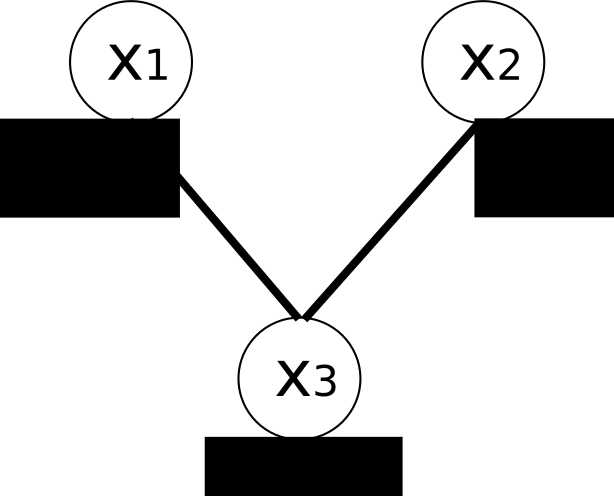
\includegraphics[width=0.7\textwidth]{DCSP}
			\caption{corresponding agent graph.}\label{dcsp:graph}
	\end{subfigure}

\caption{An example of DCSP representation.}
\label{dcsp}

\end{figure}

From this graph representation, the DCSP formalism\cite{yokoo1998distributed} models a CSP  as an agent graph, with each agent in charge of assigning a value to a variable based on local and shared constraints. A DCSP is described as a quadruplet <$X, D, C, A$>. $X, D$ and $C$ have the same meaning than in the CSP formalism, while $A$ is the set of agents. For each agent in $A$ has the responsibility of a subset of $X$ and knows the constraints related to the variables in its care. The most common assumption is that each agent has the responsibility for one and only one variable. See \figurename{} \ref{dcsp} for an illustration of the graph transformation of a DCSP.

One classical example of DCSP solver is Asynchronous Backtracking (ABT) \cite{Yokoo:2001:DCS:380145}. ABT creates a total ordering on the agents and models the relations between agents as directed links, in order to make the network cycle-free. In ABT agents exchange \emph{nogoods}, which are conditional constraints (the constraint is valid as long as other agents do not change states). When an agent detects a \emph{nogood}, it checks if it can change its state in order to solve it. If it is possible it does so and informs the agents to which it is linked. Else it propagate it to the lowest priority agent it knows (based on the established ordering) involved in the \emph{nogood}, creating new links if necessary.

An extension of DCSP has been proposed for formalizing Distributed Constrained Optimization Problems (DCOP, or DisCOP). DCOP is to COP the equivalent of DCSP to CSP. While a DCOP is described in the same way than a DCSP, the semantic and goal are different.
In DCOP, the constraints in $C$ represent a decomposition of a global cost function, which the agents try to minimize (or alternatively, maximize). Each constraint is now seen as a local cost function giving the cost associated with each state of two variables (in the context of DCOP, the term \emph{constraint} is sometimes replaced by the terms \emph{cost function} or \emph{soft constraint}). Formally, DCOP considers the global objective-function $F(X) = \displaystyle\sum_{x_i, x_j \in X} c_{ij}(x_i,x_j)$ where $c_{ij}$ is a local cost function associated with the states of $x_i$ and $x_j$.

A classical use of DCOP is unsolvable CSP[[s]], problems where there is no solution which satisfies all the constraints. In these cases the problem can be changed into a DCOP with the new objective to minimize the number of violated constraints. If we wanted to transform the problem shown in \figurename{} \ref{dcsp} (ignoring the fact that this DCSP is in itself solvable), we could replace the constraints in $C$ by the function $c_{13}$ and $c_{23}$ defined as follows:

\begin{center}
\begin{tabular}{ccc}
\toprule
$\boldsymbol{x_1}$	& $\boldsymbol{x_3}$ & $\boldsymbol{c_{13}(x_1,x_3)}$\\
\midrule
0   & 0	& 1\\
1   & 0	& 0\\
0   & 1	& 0\\
1   & 1	& 1\\
0   & 2	& 0\\
1   & 2	& 0\\
\bottomrule
\end{tabular}
\quad
\begin{tabular}{ccc}
\toprule
$\boldsymbol{x_2}$	& $\boldsymbol{x_3}$ & $\boldsymbol{c_{23}(x_2,x_3)}$\\
\midrule
1   & 0	& 0\\
2   & 0	& 0\\
1   & 1	& 1\\
2   & 1	& 0\\
1   & 2	& 0\\
2   & 2	& 1\\
\bottomrule
\end{tabular}
\end{center}

In the context of this framework, many techniques have been proposed. One of the leading algorithms to date is the Asynchronous Distributed Optimization Algorithm (ADOPT) \cite{Modi06adopt:asynchronous}.In order to work, ADOPT needs to reformulate the problem by introducing a total ordering on the agents. This ordering allows to create a tree representation of the problem, where each agent has a single parent and multiple children. The algorithm in itself is articulated on two main ideas:

\begin{compactitem}
\item each agent asynchronously changes states when it perceives a possible better solution.
\item the agents can backtrack to previously explored solutions, but only if this current state is worse than a specific \emph{backtrack threshold} determined by its parent agent.
\end{compactitem}

Another well-known algorithm is Optimal Asynchronous Partial Overlay (OptAPO) \cite{Mailler-355}. this algorithm is an adaptation of Asynchronous Partial Overlay (APO), which was proposed for solving DCSP. OptAPO, as APO, is based on the principle of \emph{Cooperative Mediation}, where the agents try to identify parts of the problems which can be solved in a centralized way (using centralized solvers such as Branch-and-Bound). During solving, some of the agents take the role of mediator during \emph{mediator sessions}, where they compute a solution to a part of the whole problem and propose solution to the others agents involved into the mediation.

The DCOP formalism is very popular in its own right as it allows a clear framework on how to represent this type of combinatorial problems without putting too much restriction on how the problem  is solved. The exact information shared by the agents, and the way they communicate among themselves is not constrained. However this formalism is not without limitations.\\
While some works successfully used DCOP in the context of continuous optimization\cite{stranders2009decentralised}, this formalism is not adequate to handle the full range of continuous optimization problems. DCOP was conceived for a specific type of problems where the difficulty resides in the combination of multiple constraints. These problems are supposed to be easily decomposable into several cost functions, where the cost values associated to the variables states are supposed to be known. This major assumption does not stand for complex continuous optimization problems (such as MDO problems for example), where the complexity of the models and their interdependencies cause this information to be unavailable in most cases. Modeling such problems with DCOP would be impossible in most case, as most agents would potentially be related to every other agent and the cost functions would be unknown.

It is interesting to note that many methods require non-trivial changes to the topology of the agent graph to work (acyclic graph, tree structure ...), both in the context of DCSP and DCOP. These changes can  be potentially extensive operations in themselves, and must be applied carefully lest the relevance of the results be compromised. Consequently, most existing agent-based optimization techniques for DCOP may require a strong expertise to be efficiently applied\cite{Ka2011.6}.

\subsubsection{Multi-Agent Systems for Continuous Optimization}

While MAS are a popular approach for solving combinatorial optimization problems, their application to continuous optimization problems is scarce at best. One could explain this discrepancy by the fact that continuous optimization problems are in general more difficult to decompose than combinatorial ones.

As said in the previous section, an adaptation of DCOP with continuous variables has been proposed in \cite{stranders2009decentralised}. This work proposes an adaptation of the max-sum algorithm in the continuous case by redefining the two operations of summation and maximization in order to be able to use them over continuous utility functions. However, this work concentrates on a specific type of problem (distributed sensor networks) and the utility functions must be piecewise linear. It is not applicable to broader scope of continuous optimization problems which concern us here.

Some works have been proposed for using MAS for dynamic continuous optimization (see \cite{lepagnot2010new} for example). However these works usually base their approach on population-based exploration of the search space, where one agent represents a single candidate solution of the problem. These kinds of population-based approaches are ill-suited for complex problems, where a major difficulty is the cost of evaluating a point in itself.

A notable work on the subject of general continuous optimization is the MASCODE algorithm \cite{welcomme2006self}, which concentrates on MOO and MDO problems. In MASCODE, each agent is in charge of a discipline and the links between agents represent the dependencies between the different disciplines. For each input of a discipline, a \emph{physical validity interval} and an \emph{objective validity interval} are defined. These two intervals represent respectively the physical constraints of the model and the boundaries of an objective to achieve. Using these two measures, a satisfaction measure is defined using a parametric piecewise continuous function. The basic idea of this satisfaction measure is as follows: 
\begin{compactitem}
\item when the value of the input is in the boundaries of the objective validity interval, the satisfaction of the agent regarding this input is high,
\item when the value of the input is outside of the objective validity interval but inside the physical validity interval, the satisfaction lowers,
\item if the value of the input goes outside the physical validity interval, the satisfaction becomes minimal.
\end{compactitem}

The agents use the values of their inputs to send \emph{forward messages}, informing others agents of the values of their outputs. Upon reception of these messages, an agent uses these new values to recalculate its own outputs (potentially sending in turn new \emph{forward messages}) and send \emph{backward messages} to the agents controlling their inputs. These \emph{backward messages} are modification requests indicating the satisfaction of the requesting agent. Upon reception of such messages, the agent will select which ones to handle based on the current satisfaction degree of their sender and will change the value of its inputs accordingly (sending in turn new \emph{backward messages} if required).

This algorithm is very interesting as it makes very few presuppositions concerning the shape of the optimization problem. The problem can be expressed as initially conceived by the designer, without requiring special transformation operations. Still, there are some limitations to the expressiveness of the formulation. The possibilities for the designer to express constraints and objectives of the problem are restricted to the specific use of the physical and objective validity intervals. As a consequence, constraints and objectives cannot be expressed independently, and can only concern \emph{one} variable at a time. While this latter limitation can somewhat be circumvented by introducing artificial disciplines placeholders, the natural modeling of the domain is then lost. This limitation can be explained as a consequence to the specific application domain which was considered for the algorithm (industrial product design).

\subsubsection{Analysis of Multi-Agent Systems for Distributed Problem Solving}

We have seen in this section how MAS have been applied for problem solving. While the solving of discrete constraint satisfaction and optimization problems has been a very popular topic of interest, very few works exist concerning the solving of continuous problems. Among the few existing works, most concentrate on specific application topics, thus no real unified effort exist in this regard comparable to one which can be observed for discrete optimization.

One of the main contributions of this thesis is to rectify to this deficiency by providing not only an agent based method for general continuous optimization but also a general modeling for enabling further contributions on a comparable basis.

\section{The Adaptive Multi-Agent Systems Theory}\label{amas_theory}

\subsection{Theorem of Functional Adequacy}

The design of a MAS for problem solving is not an easy endeavor. We can observe that most of the MAS algorithms dedicated to problem solving proposed by the scientific community are nature-inspired (ants, flocks, bees, bats etc.) \cite{di2011self}. Indeed, Nature had a long time to experiment on several arduous problem and plenty of subjects at hand. Why would we not take advantage of that? However, such a strategy presents a severe limitation, as it can bring us existing solutions to apply to potential problems, but ultimately cannot help us to find potential solution to some existing problems. By restricting ourselves to nature-inspired mechanisms we are bound to their application field.\\
%The inspiration for things such as the internal combustion engine was not found in nature, since no other biological organism than men ever bothered with something in appearance so foolish as trying to reach for the Moon\footnote{In total honesty, it is possible that some other organisms already tried to reach for the Moon. But it seems such behavior did not give them enough significant evolutionary advantage to be noteworthy (except of course for a specific cow in the popular nursery rhyme \cite[p.~203--204]{opie1997oxford}).}.

In order to overcome this limitation, we need to rely on a more theoretical approach which would help us in the design of MAS for which we do not know any existing applicable mechanisms. Such an approach is provided by the Adaptive Multi-Agent Systems (AMAS) theory.

The AMAS theory was developed by the SMAC team and formalized in \cite{glize2001adaptation}. It focuses on cooperation as the fundamental mechanism of MAS design.

%This modeling is holonic \cite{koestler1989ghost} at its core, since the agents themselves can also be viewed as systems for which the environment consists of the other agents and the environment of the encompassing system.

At the basis of the theory is the modeling of a system as a set of entities, the agents, interacting with each others and with their environment. The system can be deemed to be \emph{functionally adequate} by an external observer if this latter judges that the system as a whole correctly accomplishes its function in regard to the environment. This external observer can be considered to be a perfect oracle, in a way similar to the Laplace's demon, knowing exactly which will be the consequences of each interactions between the system and its environment.

It is important to understand that, from a theoretical point of view, the notion of functional adequacy is inherently subjective, and depends on the observer. In practice it is however usually easier to attain a reasonable consensus. For example a natural system will usually be deemed adequate if it survives and thrives in a sustainable way. For an artificial system it is often even easier since the functional adequacy correspond to the function expected by the designer of the system.

The AMAS theory identifies three categories of interactions between a system and its environment:
\begin{compactitem}
\item Cooperative action: the acting entity is beneficial to the other.
\item Antinomic action: the acting entity is detrimental to the other.
\item Neutral action: the acting entity has no effect on the other.
\end{compactitem}

From this categorization, the theory draws its formal definition (and fundamental axiom) of functional adequacy:

\definition{Axiom of functional adequacy}{A functionally adequate system has no antinomic interaction with its environment}

\begin{figure}
\centering

	\begin{subfigure}[b]{0.45\textwidth}
		\centering
		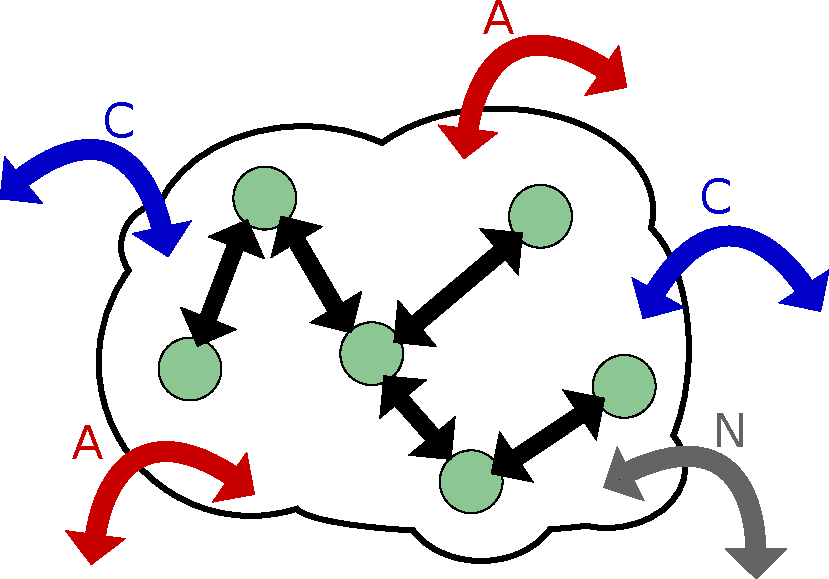
\includegraphics[width=\textwidth]{system_non_adequate}
		\caption{non functionally adequate system.}\label{adequacy_comp_1}
	\end{subfigure}
	\begin{subfigure}[b]{0.45\textwidth}
		\centering
		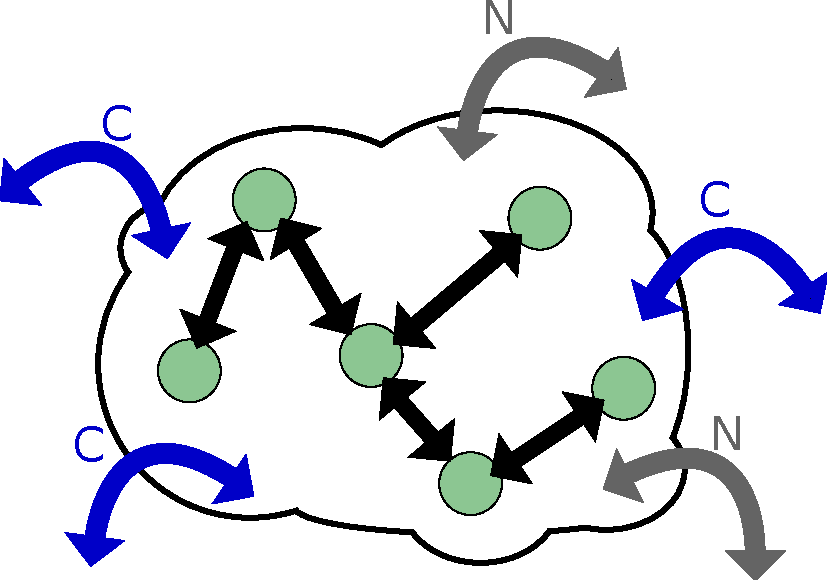
\includegraphics[width=\textwidth]{system_adequate}
		\caption{functionally adequate system.}\label{adequacy_comp_2}
	\end{subfigure}
	
	\begin{subfigure}[b]{0.45\textwidth}
		\centering
		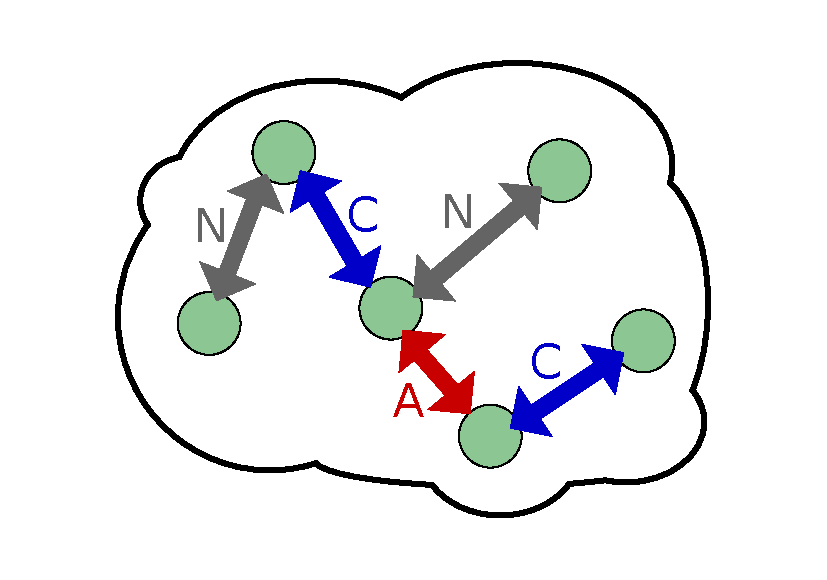
\includegraphics[width=\textwidth]{system_non_cooperative}
		\caption{non internal cooperative medium system.}\label{internal_cooperative_comp_1}
	\end{subfigure}
	\begin{subfigure}[b]{0.45\textwidth}
		\centering
		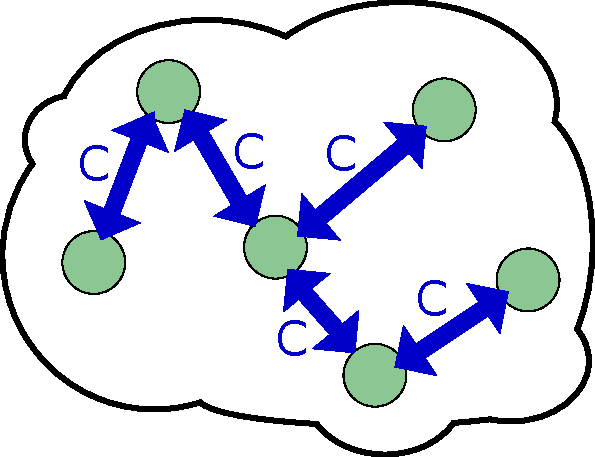
\includegraphics[width=\textwidth]{system_cooperative}
		\caption{internal cooperative medium system.}\label{internal_cooperative_comp_2}
	\end{subfigure}
	
	\begin{subfigure}[b]{0.7\textwidth}
		\centering
		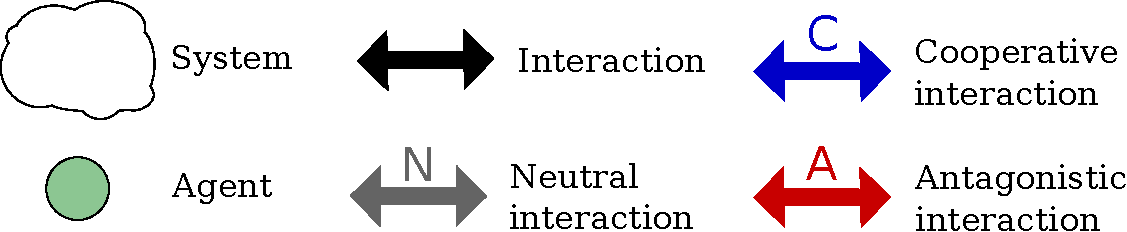
\includegraphics[width=\textwidth]{system_legend}
	\end{subfigure}
	
\caption{Illustration of functionally adequate  and internal cooperative medium systems.}
\label{adequacy_comp}
\end{figure}

An illustration this axiom is shown on \figurename{} \ref{adequacy_comp_1} and  \figurename{} \ref{adequacy_comp_2}.


%\definition{Internal cooperative medium system}{A system in which the agents only have cooperative interactions with each others or their environment[[?]]}

Using this axiom, several properties have been demonstrated concerning a specific set of \emph{internal cooperative medium systems}, defined as systems in which the agents do not have any antinomic or neutral interaction (illustrated on \figurename{} \ref{internal_cooperative_comp_1} and \figurename{} \ref{internal_cooperative_comp_2}). We will not enter here in the details of these properties and their demonstration, the interested reader can refer to \cite{glize2001adaptation, gleizes1999theory}. It suffice to say that these properties lead to the central theorem of functional adequacy:

\definition{Theorem of Functional Adequacy}{For each functionally adequate system there exists an internal cooperative medium system also functionally adequate in the same environment}

This theorem is at the core of the AMAS approach of system design. We already know that for each problem there is possibly an infinity of equivalent systems producing the same adequate functioning. Using the theorem of functional adequacy we can concentrate on designing an internal cooperative medium system, that is, designing a system were the agents cooperate among themselves and with their environment. The goal of a designer using this approach is thus to study the nature of the interactions between the entities of the problem domain, and to see how the non cooperative situations could be corrected in order to obtain an internal cooperative medium system.

In addition to providing us with a theoretical context, this approach gives us another interesting property: as the design of the system is focused on the local interactions of the agents, we do not need to explicitly take into account the global function of the system. This property is extremely significant. If the global function is complex, it can be extremely difficult to successfully design a system which explicitly tries to achieve the global function (top-down approach). By concentrating on the local functions of the agents, we can spread the complexity and ease the design of the system (bottom-up approach). As such, this approach strongly relies on the emergence phenomenon and is often referred to as \enquote{Emergent Problem Solving} \cite{quinqueton2000emergent}.

\subsection{Cooperative Agents and Non Cooperative Situations}

To guide the designer during the building of such internal cooperative medium system, the conditions of what makes an agent a \emph{cooperative agent} have been further formalized. An agent is said to be cooperative if it satisfies three conditions:
\begin{compactitem}
\item $C_{perception}$ Every perceived signal can be understood without ambiguity
\item $C_{decision}$ Every interpretation must produces useful information
\item $C_{action}$ Every action done based on the decision must be useful
\end{compactitem}

Based on these conditions, a set of \emph{Non Cooperative Situations}(NCS) has been identified. These NCS[[s]] correspond to interactions which are not cooperative and must be removed for the system to be an internal cooperative medium system. The NCS[[s]] are classified based on the condition they violate. The table in \figurename{} \ref{NCS} shows this classification.

\begin{figure}
\centering
\begin{tabular}{ll}
\toprule
\textbf{Violated condition}	& \textbf{Corresponding NCS} \\
\midrule
$C_{perception}$     & Incomprehension, Ambiguity\\

$C_{decision}$      & Incompetence, Unproductiveness \\

$C_{action}$     & Uselessness, Competition, Conflict\\
\bottomrule
\end{tabular}
\caption{The conditions for cooperation and corresponding NCS}
\label{NCS}
\end{figure}

The different NCS are:
\begin{compactitem}
\item\textbf{Incomprehension} The agent is not able to extract information from a received message.
\item\textbf{Ambiguity} The exact meaning of a message cannot be determined, or lacks required informations.
\item\textbf{Incompetence} The agent does not have the capabilities to handle a received information.
\item\textbf{Unproductiveness} A received information does not lead to any useful conclusion.
\item\textbf{Conflict} The action of the agent is incompatible with an action from its environment.
\item\textbf{Competition} The action of the agent leads to the same result than an action from its environment.
\item\textbf{Uselessness} The action of the agent has no effect on itself or its environment.
\end{compactitem}

A cooperative agent actively tries to avoid these NCS and, should this fail, to solve them to the best of its capabilities. To this end, three distinct mechanisms can be used\cite{bonjean2009engineering}:

\begin{compactitem}
\item\textbf{1. Tuning} The agent can change one or several of its internal parameters (\textit{e.g.}, adjusting the priorities of its behavior rules).
\item\textbf{2. Reorganization} The agent can change its relationship with its environment (\textit{e.g.}, removing or creating new links with others agents).
\item\textbf{3. Evolution} The agent can change the nature of its environment (\textit{e.g.}, removing or creating new agents).
\end{compactitem}

The order of these mechanisms usually correspond to their level of disruption (\textit{i.e.}, adjusting its parameters usually has less consequences than creating and removing agents). In general, it is preferable to make the less disruptive possible adjustment. One can for example design the agents based on an escalation principle, where the agents try to solve NCS first by using tuning, escalating to a more disruptive mechanism only when the previous ones failed to solve the NCS. Of course, a NCS situation being by itself disruptive, it is sometime more efficient to immediately make a more radical adjustment in order to solve the NCS more quickly. The designer will have to balance these concerns according to the specificities of the system.

\subsection{The Importance of Locality}

A primordial aspect of the AMAS theory is the importance of locality. The theory insists on the need to consider and consider only the partial knowledge and local interactions between the agents, without trying to provide a \enquote{bigger picture}. While this concern can be linked to specific notions like the concept of emergence, we believe that a direct explanation can be found regarding preoccupation about the \emph{scalability} of the system.

The AMAS theory concerns systems which aim to solve complex problems. By definition the difficulty of such problem increases exponentially with its size. To design a MAS able to scale with the size of the problem, the designer has in general two possibilities: he can increase the size of the system or increase the complexity of the agents. The key difference between these two operations is their marginal costs. While adding a new agent to the system should usually represent a constant cost (in terms of complexity, computational requirements ...), increasing the complexity of the agents will be more and more difficult, since the agents will individually reach the same limitations as centralized methods. The principle of locality is a good example for this argument. Suppose a hierarchical system where one of the agent is in charge of a whole subsystem. If the increase of the complexity of the problems results in an increase of complexity of the subsystem, after some limits the agent will not be able to handle correctly the subsystem, resulting in a limit to the scalability of the system as a whole.

The software engineer will not miss the uncanny similarity of this argument with the relatively recent trend regarding scalability concerns for computer infrastructures (for \emph{e.g.} web servers, distributed databases \emph{etc.}). The two main categories for scaling resources in such systems are \emph{vertical scalability} (scaling \enquote{up}) and \emph{horizontal scalability} (scaling \enquote{out}). Vertical scalability is the improvement of existing resources for them to be able to handle more data/traffic/..., while horizontal scalability consists in adding more resources to spread the workload. While in the past vertical scalability was the dominant practice, the current consensus seems to be that horizontal scalability is easier and provides better performances increase \cite{michael2007scale}.\\
Of course such comparison must be made with caution, as the context of the two fields are quite different. However it is interesting to note how similar concerns from these different fields led to a similar evolution in the approaches.

Obviously, such general principles cannot hold systematically true and some problems which cannot be solved by adding more agents are easily resolved by improving their reasoning capabilities. More so, in some cases increasing the size of the system can increase the complexity of the existing agents (for example by adding neighbors to an agent, thus increasing the complexity of its decision process). Still, in the general case, the motto of approaches such as the one of the AMAS theory could be \enquote{scale out when you can, scale up when you must}. 

\subsection{ADELFE - A Method for Designing AMAS}\label{AMAS-ADELFE}

ADELFE \cite{bernon2003adelfe} is a method dedicated to the development of AMAS. The name \enquote{ADELFE} is the French acronym for \enquote{toolkit to develop software with emergent functionality} (\textit{Atelier pour le DEveloppement de Logiciels à Fonctionnalité Emergente}). While ADELFE is not the only method devoted to guide the design of a MAS, its specificity concerns the fact that it is specifically tailored for AMAS.

The ambition of ADELFE is to provide be-all and end-all method to guide engineers during all the phases of the design of an AMAS, from the high-level requirements to the \enquote{nuts and bolts} implantation details. This ambition was the driving factor for multiple projects with the objective of improve or complement ADELFE with additional tools, such as the Make Agents Yourself (MAY) framework  \cite{No2012.2}, used to automatically generate agent architecture implementations.

However, as for most general engineering methods, a current limitation of ADELFE is that it only provide high-level guidelines concerning the behavior and architecture of the agents, staying at a general, abstract level. This current limitation makes difficult for a non-expert in AMAS to actually provide an adequate instantiation for the problem he wants to solve. It is the same analysis in \cite{Ka2011.6} which led the author to prone a specialized variant of the method containing additional guidelines and tools for applying AMAS in the context of problem solving.

We will go into greater details concerning the inner workings of ADELFE and how this method was involved in the context of this thesis in chapter \ref{ADELFE_chapter}.

\subsection{Conclusion on the Adaptive Multi-Agent Systems Theory}

We presented here the AMAS theory. This theory presents a way to model systems by their constituting parts, the interactions between themselves as well as with the environment and identify the special category of internal cooperative medium systems.

An interesting aspect of this theory  is that it provides a guidance to build a multi-agent system based on the problem to solve. Classical solving methods often use a very rigid formalism which needs to be followed. For example, genetic algorithms are a very powerful technique, but they require the problem to fit the genetic representation/fitness function model. To use these kinds of methods, one would now be presented to a whole new problem: \enquote{how can I express my problem to fit the solution I want to employ ?}

While a non-negligible part of real-world problems are more or less straightforwardly translatable in such formalisms, there is still a whole range of problems for which this translation is not so easy. This can be either because no method adequate enough for the domain was proposed, or because there is no consensual representation of the domain. For these problems, the AMAS theory can provide an interesting asset as the design of the MAS is based on the problem domain. The solution is adapted to the problem, instead of requiring the problem to be adapted to the solution.

We can say that, while the AMAS approach can be applied to any kind of problem, it seems to be especially adequate when trying to solve problems which are still in an exploratory phase, where no \enquote{clear-cut} solution exists.


